\section{Visualization and Event Display}
\label{sec:display}

Visualization of raw and reconstructed data provides essential information to assist experimenters in multiple tasks:

\begin{itemize}
    \item \textbf{Algorithm development -} tracks or clusters from alternative algorithms can be visualized within the geometries and alongside Monte Carlo truth information, allowing easy comparisons and aiding debugging
    \item \textbf{Simulation studies -} Monte Carlo information can be visualized, allowing studies of particle interactions in instrumented or uninstrumented detector regions
    \item \textbf{Detector commissioning -} during initial commissioning sub-systems will be tested independently, sometimes in incomplete configurations. Visualizing of through-going cosmic rays can provide useful information to detector teams
    \item \textbf{Physics analysis -} visualization of data within the detector systems can provide invaluable information about the nature of an event. In the event of a signal-like track, the collaboration we will want to explore in great detail the properties of this event, and the event display will be a key tool.
\end{itemize}

Three event displays are currently available. The first is a custom ROOT-based display showing geometries and data products as TGeo objects. The second is TEveMu2e, exploiting ROOT's existing Event Visualization (EVE) framework, TEve. This framework allows visualization of all detectors via the ROOT OpenGL interface. The full Mu2e geometry can be imported into TEve via a simple GDML file. In addition to the main 3D display, users can browser-specific 2D views of each detector system via tabs in the browser. A third display, REveMu2e, is based on ROOT's REve class~\cite{Tadel:2020hlt}. REve is an evolution of TEve for the ROOT-7 era, designed upon information collected by the HEP Software Foundation Community White Paper on Visualization~\cite{Bellis:2018hej}. It is developed by members of the CMS collaboration and will be maintained throughout the coming decade and beyond. REve utilizes the OpenUi5 (\url{https://openui5.org/}) framework to build a customizable web-based GUI, providing more modern infrastructure. A REve-based display can be set up remotely via a web browser and an SSH tunnel, allowing fast and secure operation of the viewer. REveMu2e is the default event viewer within the Mu2e experiment, and it has been integrated into the DAQ system to serve as an online event monitor during data taking.


\subsection{REveMu2e}

REveMu2e displays the entire Mu2e geometry (read from a gdml file) and all reconstructed and truth-level data products in the tracker, calorimeter, and CRV. The detector display in the "extracted position" during the commissioning phase is also supported. The user can navigate to a chosen event (this is directional as backward navigation is prohibited in art) and rotate, zoom, and pan the view. 

The code is structured in sets of "scenes" containing different types of information. The geometry scenes include individual detector geometry objects, such as the tracker or CRV scenes, allowing users to add or remove sub-systems from the display interactively. The event "scene" contains event-by-event information on physical objects: REveLines for trajectories and REvePointSets for hits or clusters. Within this scene, objects of interest can be highlighted. For example, the color of the crystal and its length is proportional to the energy deposited in that crystal. The display can also show GEANT4 trajectories, allowing offline analysts to compare their reconstruction with Monte Carlo truth information. Information associated with a given data product can be obtained by simply scrolling over the product. Interactive labels will then pop up with various data, such as the algorithm used to reconstruct the object, its position, time, energy, etc. The GUI also provides options to print further details to the terminal. In addition, a set of 2d views is provided by default: an XY and YZ view of the tracker with XY views of each calorimeter disk. Additional views can easily be added if necessary. Illustrations of the capabilities of REveMu2e are shown in Fig.~\ref{fig:teve_3D_label} and \ref{fig:teve_3D_extracted}. 

\begin{figure}[htb]
\begin{center}
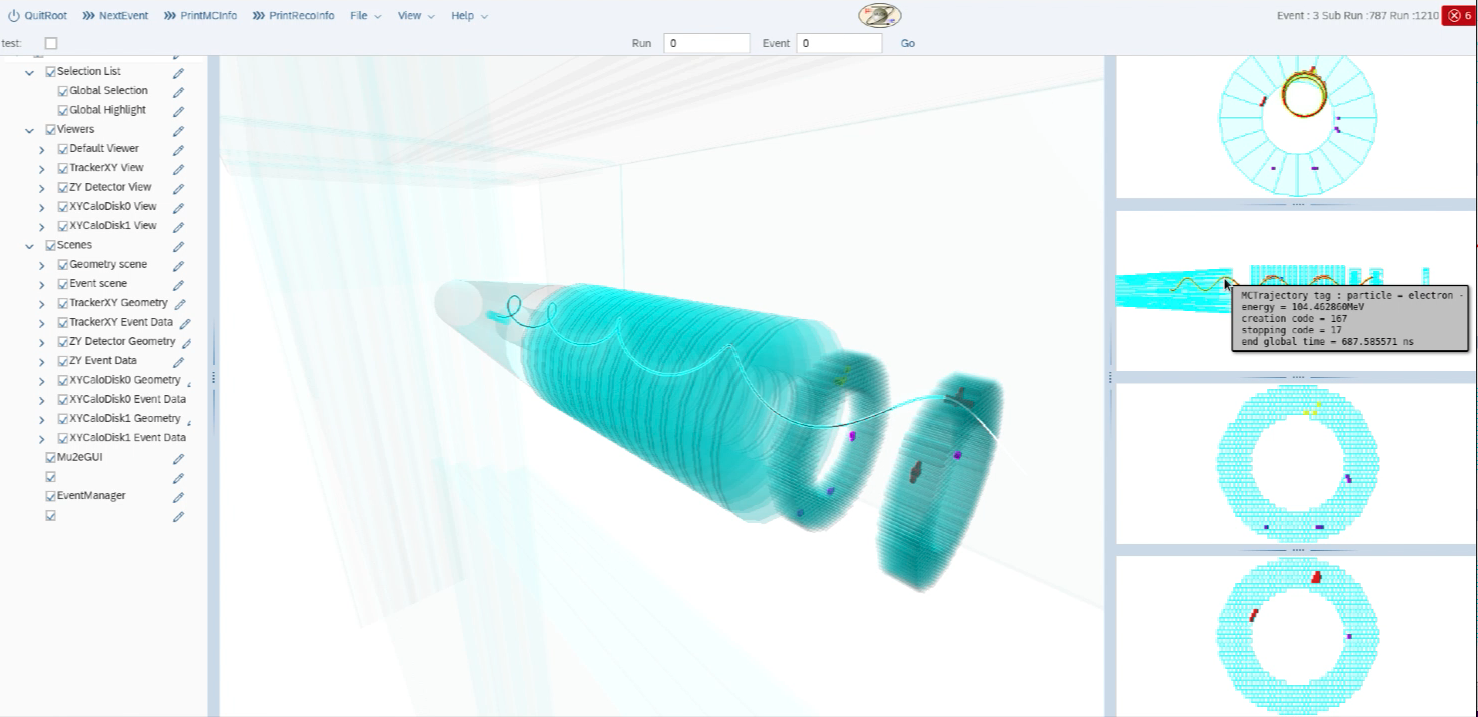
\includegraphics[width=0.9\linewidth]{figures/2D-REve-label.png}
\caption{\textbf{User Experience:} An example REveMu2e displaying a conversion entering the detector region and producing a helical track in the tracker and calorimeter. The MC truth trajectory is highlighted and a label is visible.}
\label{fig:teve_3D_label}
\end{center}
\end{figure}

\begin{figure}[htb]
\begin{center}
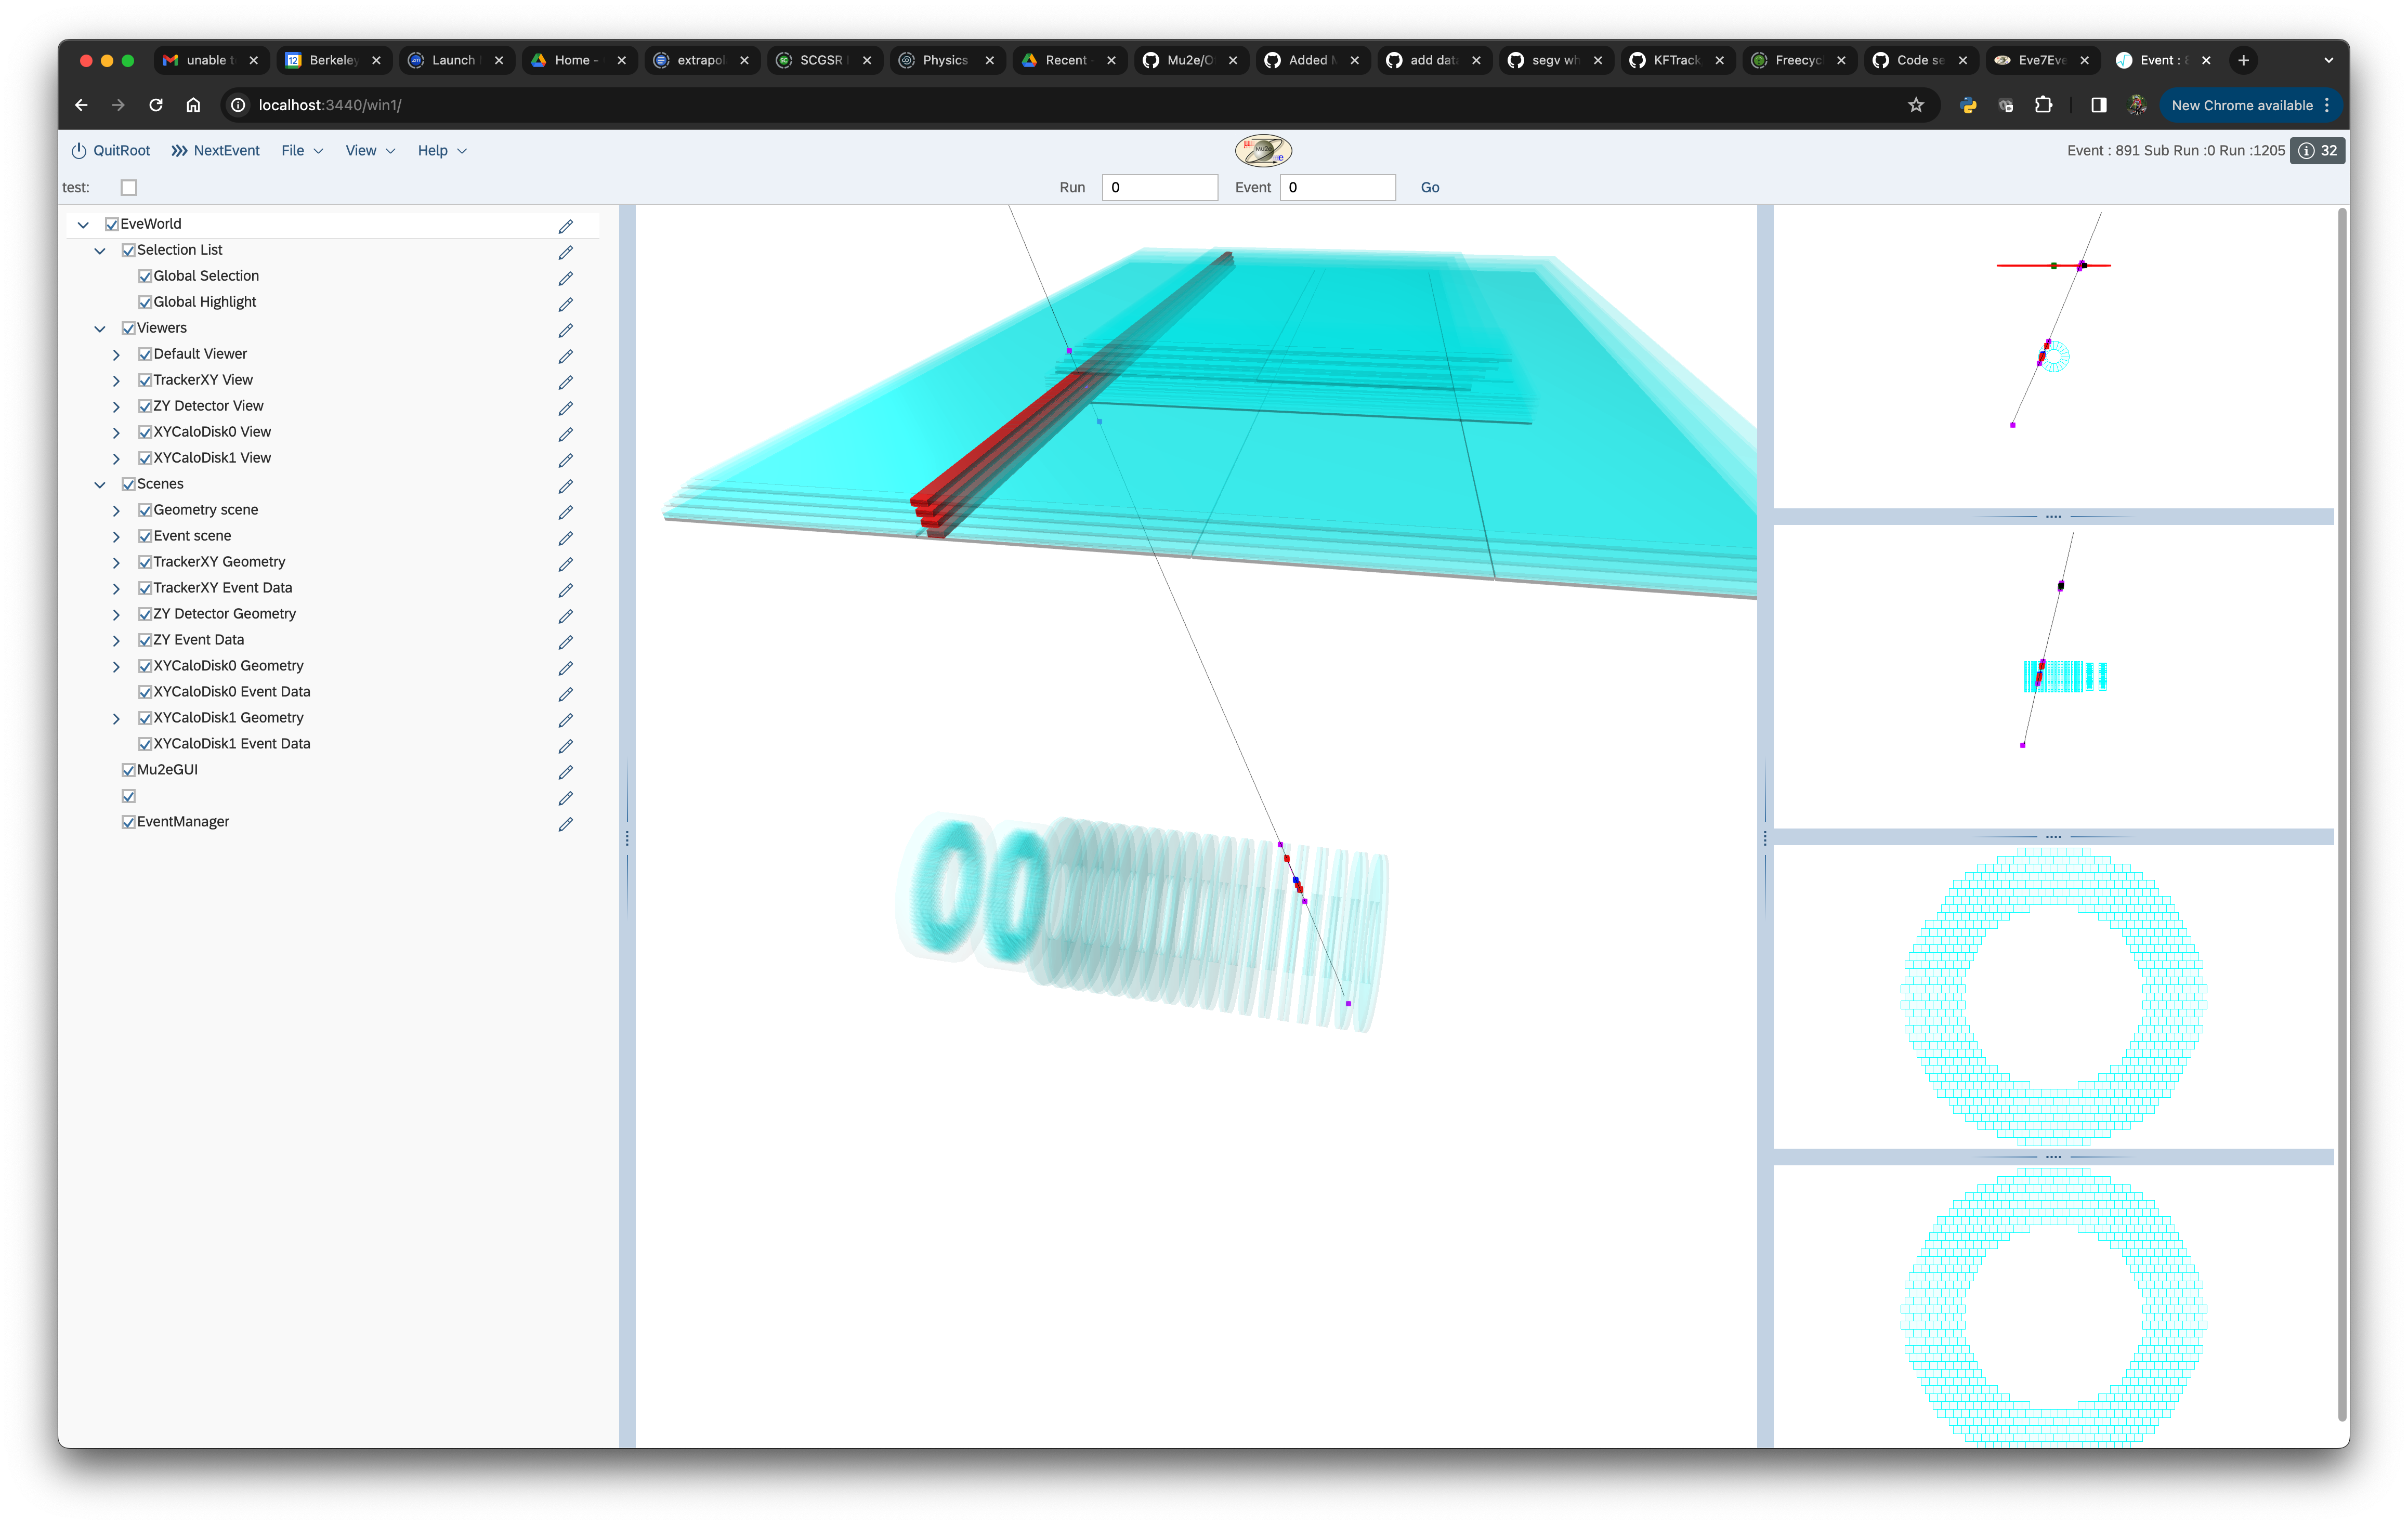
\includegraphics[width=0.9\linewidth]{figures/extracted.png}
\caption{\textbf{Extracted Cosmic View:} An example REve displays of the showing a cosmic muon entering the detector region in extracted (field off) configuration}
\label{fig:teve_3D_extracted}
\end{center}
\end{figure}

















